\chapter{Diseño del sistema de carga multiquímica}

\section{Convertidor reductor}

Para el sistema de carga multiquímica es necesario poder proporcionar una 
corriente constante para la carga de ambos tipos de baterías. Para ello
se decidió emplear un convertidor reductor, el cual tiene por componente principal
el circuito integrado LM2596. Para poder realizar un control del voltaje de salida ( y de
forma indirecta la corriente del mismo)
de forma electrónica, es decir aplicando un voltaje, se realizó una modificación al circuito
de realimentación del circuito como es mostrado en la figura \ref{fig:buck_modificado}.

\begin{figure}[H]
    \centering
    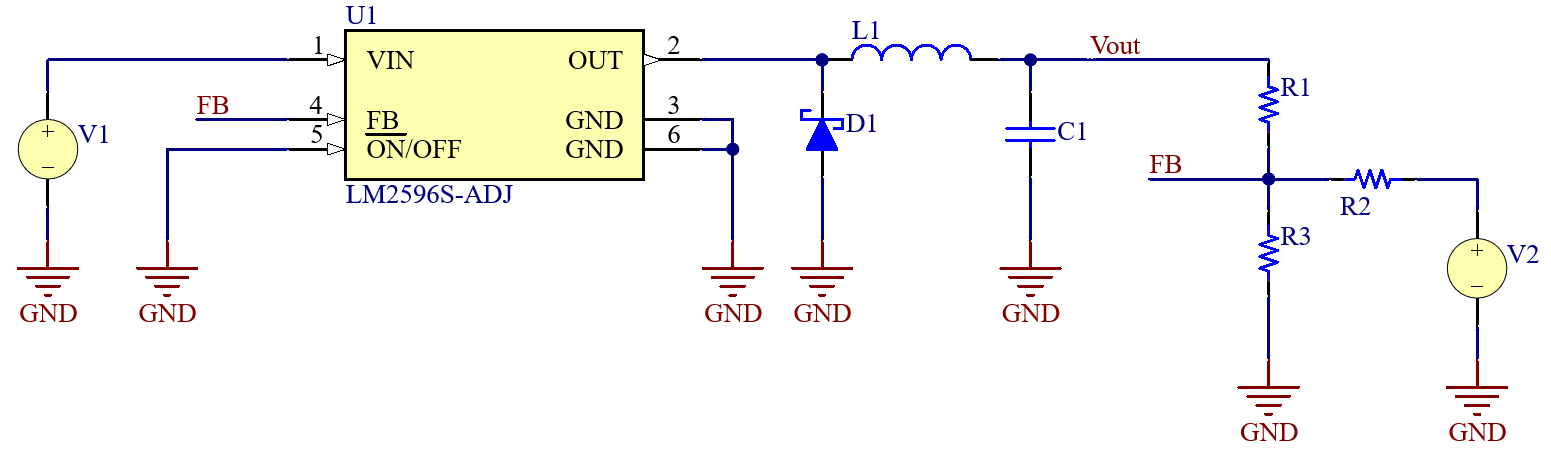
\includegraphics[scale=0.35]{imagenes/buck_control_simplificado.png}
    \caption{Convertidor reductor con realimentación modificación (versión simplificada) }
    \label{fig:buck_modificado}
\end{figure}

Para poder determinar en que forma va a variar el voltaje en el nodo $V_{out}$ se realizó un 
análisis de nodos en el nodo FB, obteniendo la ecuación \ref*{eq:buck_control}.

\begin{equation}
    V_{FB} = \frac{R_1R_2}{R_1R_2+R_3(R_1+R_2)} V_{out} + \frac{R_1R_3}{R_1R_3+R_2(R_1+R_3)} V_2
    \label{eq:buck_control}
\end{equation}

Donde $V_2$ el el voltaje aplicado de forma externa para modificar el valor de voltaje a la salida.
De la ecuación \ref*{eq:buck_control} se puede observar que el valor de $V_{FB}$ es dependiente tanto
de $V_2$ como de $V_{out}$.

Para determinar los valores de las resistencias se armó un sistema de dos ecuaciones, fijando los valores 
de $V_{FB}$,$V_{out}$,$V_2$, y $R_1$. Los dos valores necesarios de $V{out}$ se obtuvieron fijando el 
valor minimo y máximo que podría tener a la salida el convertidor, los cuales fueron de 1.8V y 4.3V para 
el convertidor encargado de cargar la batería Li-ion,